\section{Considerações Iniciais}

A fundamentação teórica deste estudo começa com um \sigla{MS}{Mapeamento Sistemático}, cujo objetivo é identificar a interseção entre as TICs e as línguas de sinais no contexto educacional. A \autoref{section:foundation:sm} oferece um resumo deste MS, enquanto análises mais detalhadas dos estudos primários, que abrangem tanto o panorama nacional quanto internacional, estão disponíveis em nossas publicações anteriores: \citeonline{FalvoJr2020_FIE, FalvoJr2020_SBIE, FalvoJr2021_RENOTE}.

A realização deste estudo permitiu identificar \textit{gaps} tecnológicos no uso de línguas de sinais no ensino-aprendizagem, destacando a necessidade de novas pesquisas na literatura. Complementar ao MS, um levantamento bibliográfico complementar foi conduzido para explorar conceitos e TICs promissoras que possam enfrentar esses desafios. As seções subsequentes expandem essas temáticas, abordando Arquiteturas de Software (\autoref{section:foundation:arch}), OAs (\autoref{section:foundation:lo}) e ASR (\autoref{section:foundation:asr}). Fornecendo assim, a base teórica para a \textit{Speech2Learning}, uma arquitetura baseada em ASR para OAs audíveis mais acessíveis, definida em detalhes no \autoref{chapter3}.

\section{Mapeamento Sistemático: TICs e Línguas de Sinais na Educação}
\label{section:foundation:sm}

Para definir o escopo deste projeto, foi crucial realizar um estudo sistemático de literatura para identificar lacunas e oportunidades tecnológicas no processo de ensino e aprendizagem com línguas de sinais. De acordo com \citeonline{Kitchenham2007}, existem duas abordagens principais para este tipo de estudo: revisão ou mapeamento sistemáticos. Optou-se pelo MS devido à sua capacidade de apresentar evidências de um domínio de estudo em um alto nível de granularidade, agrupando-as em áreas de similaridade e identificando tendências emergentes.

O protocolo de pesquisa para o MS foi cuidadosamente definido com base em diretrizes formais  \cite{Kitchenham2007, Nakagawa2010, Zhang2011, Petersen2015}. A abordagem de \citeonline{Zhang2011} foi particularmente relevante, pois orientou a estratégia de busca e os critérios de qualidade adotados no estudo. Essa estratégia foi adaptada para aumentar o rigor do processo de pesquisa, incorporando o \sigla{QGS}{\textit{Quasi-Gold Standard}} e seguindo boas práticas recomendadas na literatura (\autoref{ms:zhang-approach}).

\begin{figure}[htb]
\centering 
\caption{Busca Sistemática Baseada em QGS.}
\label{ms:zhang-approach}
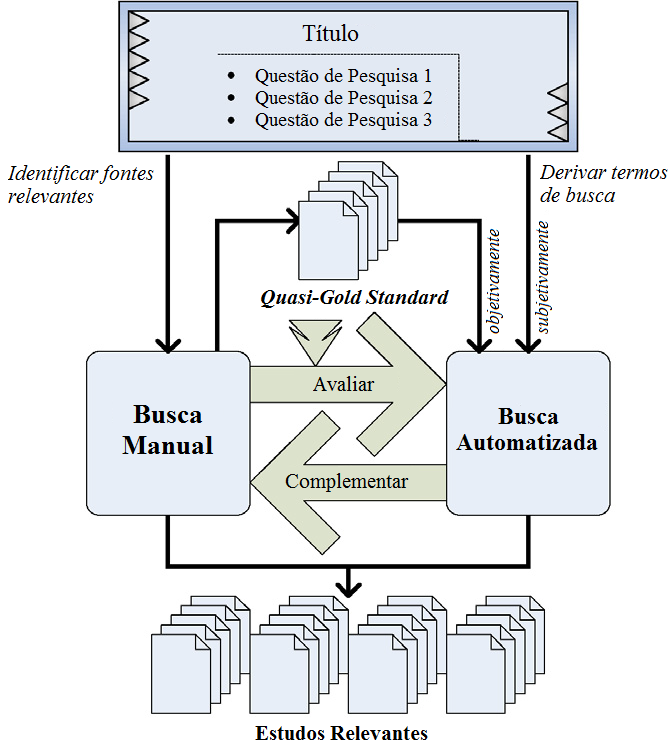
\includegraphics[width=0.675\textwidth]{images/chapter2-sm-zhang-approach.png}
\fadaptada{Zhang2011}
\end{figure}

\subsection{Definição do Escopo e Critérios de Seleção}
\label{ms:conducao-escopo}

As \sigla{QP}{Questões de Pesquisa} são essenciais para definir o escopo e identificar possíveis palavras-chave em um estudo sistemático de literatura \cite{Kitchenham2007,Petersen2015}. Neste contexto, uma abordagem comum se dá através da aplicação dos critérios de PICO \cite{Petticrew2008}. A \autoref{table:pico} representa o PICO, que derivaram as seguintes QP que definem o escopo deste MS.

\begin{table}[htb]
\centering
\caption{Critérios de PICO.}
\label{table:pico}
\begin{tabularx}{\textwidth}{lX} \hline
\textit{\textbf{P}opulation} & Aprendizes/Educadores interessados em línguas de sinais. \\
\textit{\textbf{I}ntervention} & TICs relevantes no processo de ensino-aprendizagem com línguas de sinais. \\
\textit{\textbf{C}omparison} & Não se aplica. \\
\textit{\textbf{O}utcome} & Panorama tecnológico sobre o ensino-aprendizagem com línguas de sinais. \\ \hline
\end{tabularx}
\end{table}

\begin{itemize}
    \setlength\itemsep{0em}
    \item \textbf{QP1}: Quais soluções tecnológicas vêm sendo propostas no processo de ensino-aprendizagem com línguas de sinais?
    % \begin{itemize}
    %     \item Quais são os tipos de soluções propostas (software ou hardware ou teóricas)?
    %     \item Quais tecnologias foram usadas?
    %     \item Quais métodos de avaliação foram aplicados?
    % \end{itemize}
    \item \textbf{QP2}: Quais tópicos educacionais são abordados?
    \item \textbf{QP3}: Quais línguas de sinais são abordadas?
    % \begin{itemize}
    %     \item Quais estudos abordam múltiplas línguas de sinais?
    % \end{itemize}
\end{itemize}

Segundo \citeonline{Kitchenham2007,Petersen2015}, os estudos sistemáticos requerem critérios explícitos de inclusão e exclusão para avaliar seus potenciais estudos primários. Assim, foram definimos os seguintes critérios de seleção:

\begin{table}[htb]
\centering
\caption{Critérios de Inclusão (CI) e Exclusão (CE).}
\label{tab:ms:criterios-selecao}
\begin{tabularx}{\textwidth}{lX} \hline
\textbf{CI1} & Os estudos apresentam contribuições (software ou hardware ou teóricas) para o ensino e a aprendizagem de línguas de sinais. \\ \hline
\textbf{CE1} & Estudos que não foram publicados no período de 2000 a 2019, seguindo um racional semelhante à \citeonline{Radermacher2013,Scatalon2019}, os quais sugerem que estudos anteriores a 2000 não representam as abordagens educacionais atuais, especialmente considerando o contexto de tecnologia. \\ \hline
\textbf{CE2} & Estudos classificados como resumos, resumos de conferências/editoriais, literatura cinza ou capítulos de livros. \\ \hline
\textbf{CE3} & Estudos não apresentados em inglês ou português. \\ \hline
\textbf{CE4} & Estudos não acessíveis em texto completo. \\ \hline
\textbf{CE5} & Estudos duplicados ou superficialmente complementares de outros estudos. \\ \bottomrule
\end{tabularx}
\end{table}

\subsection{Condução das Buscas Manual e Automatizada}
\label{ms:conducao-busca-manual}

No contexto das buscas manuais, a \autoref{ms:table:busca-manual-nacional} lista as conferências e periódicos nacionais analisados. No entanto, os estudos dessas fontes não foram incluídos na composição do QGS devido à limitação de indexação nos mecanismos de busca internacionais, o que poderia comprometer a eficácia da abordagem sistemática baseada em QGS \cite{Zhang2011}. Apesar disso, \textbf{46 estudos primários de fontes brasileiras foram selecionados} e discutidos nos resultados do MS. 

Por sua vez, a \autoref{ms:table:busca-manual-internacional} apresenta as conferências e periódicos internacionais selecionados durante a busca manual, resultando em 19 estudos primários que compõem o QGS deste MS. As fontes relevantes foram utilizadas para a busca automatizada, garantindo uma sinergia maior com o QGS, conforme recomendado por \citeonline{Zhang2011}.

\begin{table}[htb]
\centering
\caption{Busca Manual Nacional.}
\label{ms:table:busca-manual-nacional}
\begin{tabular}{lcc} \hline
\textbf{Conferências/Periódicos} & \textbf{Fonte} & \textbf{Selecionados} \\ \hline
DesafIE                          & CEIE           & -                     \\
JAIE                             & CEIE           & -                     \\
RBIE                             & CEIE           & 2                     \\
RENOTE                           & CINTED         & 13                    \\
SBIE                             & CEIE           & 13                    \\
WAVE2                            & CEIE           & -                     \\
WCBIE                            & CEIE           & 11                    \\
WIE                              & CEIE           & 7                     \\ \hline
\multicolumn{2}{l}{\textbf{Total}}                & \textbf{46}           \\ \hline
\end{tabular}
\end{table}

\begin{table}[htb]
\centering
\caption{Busca Manual Internacional (Equivalente ao QGS).}
\label{ms:table:busca-manual-internacional}
\begin{tabular}{lcc} \hline
\textbf{Conferência/Periódico} & \textbf{Fonte}     & \textbf{Selecionados (QGS)} \\ \hline
ACM TOCE                       & ACM                & 0            \\ 
Computers \& Education         & Elsevier           & 5            \\ 
FIE                            & IEEE               & 0            \\ 
HCI International              & Springer           & 5            \\ 
ICALT                          & IEEE               & 5            \\ 
IEEE ToE                       & IEEE               & 1            \\ 
IEEE TLT                       & IEEE               & 0            \\ 
Informatics in Education       & Vilnius University & 0            \\ 
ITiCSE                         & ACM                & 2            \\ 
Learning @ Scale               & ACM                & 0            \\ 
SIGCSE                         & ACM                & 1            \\ \hline
\textbf{Total}                 & \textbf{}          & \textbf{19}  \\ \hline
\end{tabular}
\end{table}

Tendo em vista a busca automatizada, duas estratégias para identificação de palavras-chave foram utilizadas em conjunto para nossa string de busca: (i) análise do PICO e suas respectivas QP; (ii) importação da tripla \textit{title-abstract-keywords} em um software de análise de frequência. Os resultados desse processo produziram a seguinte string de busca (\autoref{codigo:string_busca_ms}).

\begin{codigo}[caption={String de Busca do MS}, label={codigo:string_busca_ms}]
    (learn OR learning OR teach OR teaching) AND
    ("sign language" OR "signed language") AND
    (technology OR technologies)
\end{codigo}

A \autoref{method:table:automated-search} resume os resultados da busca automatizada, onde a seleção dos estudos seguiu o mesmo racional apresentado na busca manual. Além disso, a busca automatizada retornou a maioria dos estudos selecionados pela busca manual (QGS), o que sugere uma boa sensibilidade da string de busca. Nesse sentido, \citeonline{Zhang2011} propõem o conceito de \textit{quasi-sensibility}, uma derivação da sensibilidade tradicional que incorpora o QGS como critério de qualidade (\autoref{method:equation:quasi-sensitivity}).

\begin{table}[htb]
\centering
\caption{Resultados da Busca Automatizada.}
\label{method:table:automated-search}
\begin{tabular}{lllll} \hline
 &  & Busca Final &                 &                   \\ \cline{3-5} 
Base de Dados & \textbf{QGS} & Recuperados    & \textbf{no QGS} & \textbf{Relevantes} \\ \hline
ACM DigitalLibrary & 3            & 922          & 3               & 47                \\
IEEE Xplore        & 6            & 359          & 5               & 59                \\
ScienceDirect      & 5            & 1,961        & 5               & 20                \\
SpringerLink       & 5            & 4,980        & 5               & 36                \\ \hline
\textbf{Total}   & \textbf{19}  & 8,222        & \textbf{18}     & \textbf{162}      \\ \hline
\end{tabular}
\end{table}

\begin{equation}
\label{method:equation:quasi-sensitivity}
\text{\textit{quasi-sensibility}} = \frac{\text{\textit{Estudos relevantes recuperados (\textbf{no QGS})}}}{\text{\textit{Total de estudos relevantes (\textbf{QGS})}}}
\end{equation}

Como resultado, a \textit{quasi-sensitivity} calculada foi de 94,74\% (18/19), um desempenho adequado segundo \citeonline{Zhang2011}. Portanto, os 163 artigos selecionados pelas buscas (manual internacional e automatizada) foram considerados estudos primários em potencial. Nesta etapa, 24 estudos foram excluídos de acordo com os critérios de inclusão e exclusão pré-estabelecidos. A \autoref{method:figure:evaluation-refinement} organiza os \textbf{139 estudos primários selecionados pela busca sistemática baseada em QGS}.

\begin{figure}[htb]
\centering 
\caption{Resultados da Busca Sistemática Baseada em QGS.}
\label{method:figure:evaluation-refinement}
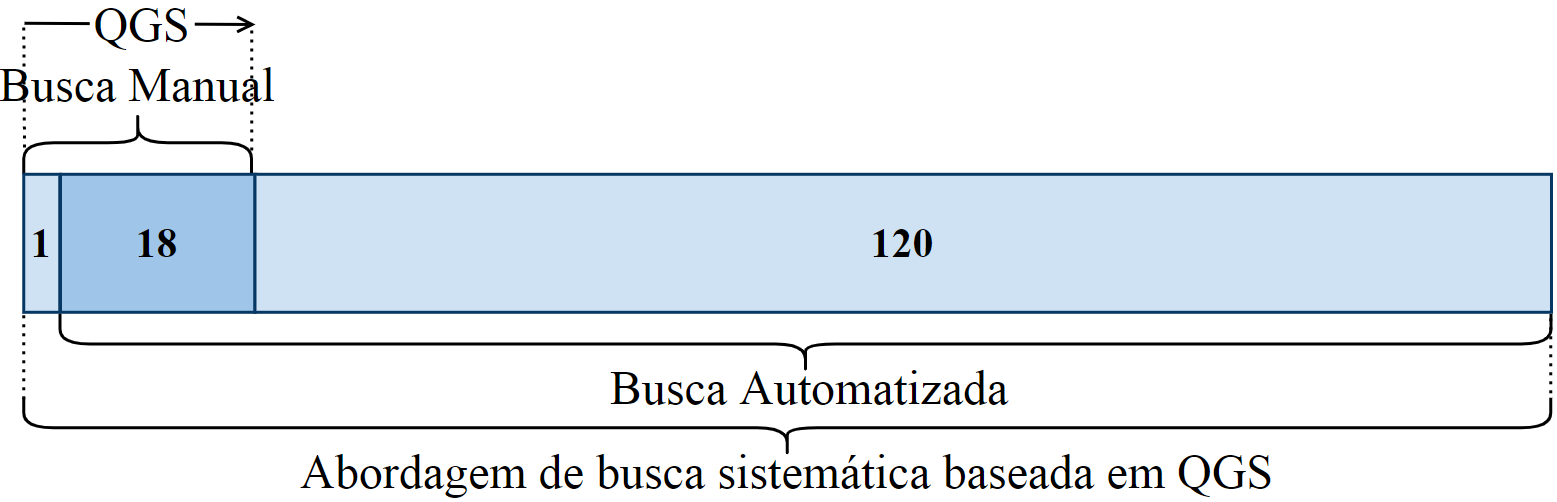
\includegraphics[width=.9\textwidth]{images/chapter2-sm-qgs-search.png}
\fautor
\end{figure}

Para extrair as informações relevantes dos estudos primários identificados, um formulário de extração de dados foi criado. A \autoref{method:table:data-extraction} representa o modelo que descreve as informações extraídas e apresenta seu relacionamento com cada QP, quando aplicável.

\sigla*{SWEBOK}{\textit{Software Engineering Body of Knowledge}}
\sigla*{ES}{Engenharia de Software}

\begin{table}[htb]
\centering
\caption{Formulário de Extração de Dados.}
\label{method:table:data-extraction}
\begin{tabular}{lll} \hline
\textbf{Item} & \textbf{Descrição} & \textbf{QP} \\ \hline
\textit{\textbf{Informações Gerais}} & & \\ \hline
ID & Identificador (prefixos \textit{INT} ou \textit{BRA}). & \\
Título & Título do estudo. & \\
Autores & Nomes dos autores. & \\
Ano & Ano de publicação do artigo. & \\
Conferência/Periódico & Nome do meio de publicação. & \\
Tipo de busca & Manual; Automatizada; Ambas. & \\
Língua & Inglês; Português. & \\
País & País da afiliação do primeiro autor. & \\ \hline
\textit{\textbf{Informações Específicas}} & & \\ \hline
Área da Eng. de Software (ES) & Área de conhecimento da ES (SWEBOK). & QP1 \\
Tipo de solução & Software; Hardware; Teórica. & QP1 \\
Estratégia empírica & Quais estratégias empíricas foram encontradas. & QP1 \\
Tópico educacional & Quais tópicos educacionais foram encontrados. & QP2 \\
Línguas de sinais & Quais línguas de sinais foram encontradas. & QP3 \\ \hline
\end{tabular}
\end{table}

\subsection{Resultados e Discussões}
\label{ms:resultados}

Portanto, o MS contou com 185 estudos primários selecionados: 46 da busca manual nacional e 139 da busca sistemática baseada em QGS. Lembrando que, as informações mais relevantes para responder cada QP foram obtidas por meio do formulário de extração de dados. Primeiramente, considerando a quantidade de publicações por ano, uma linha de tendência linear crescente foi identificada (\autoref{results:figure:publications-year}). Portanto, é estatisticamente possível que este domínio de pesquisa esteja em ascensão globalmente.


\begin{figure}[htb]
\centering 
\caption{Linha de Tendência Linear Crescente de Publicações por Ano.}
\label{results:figure:publications-year}
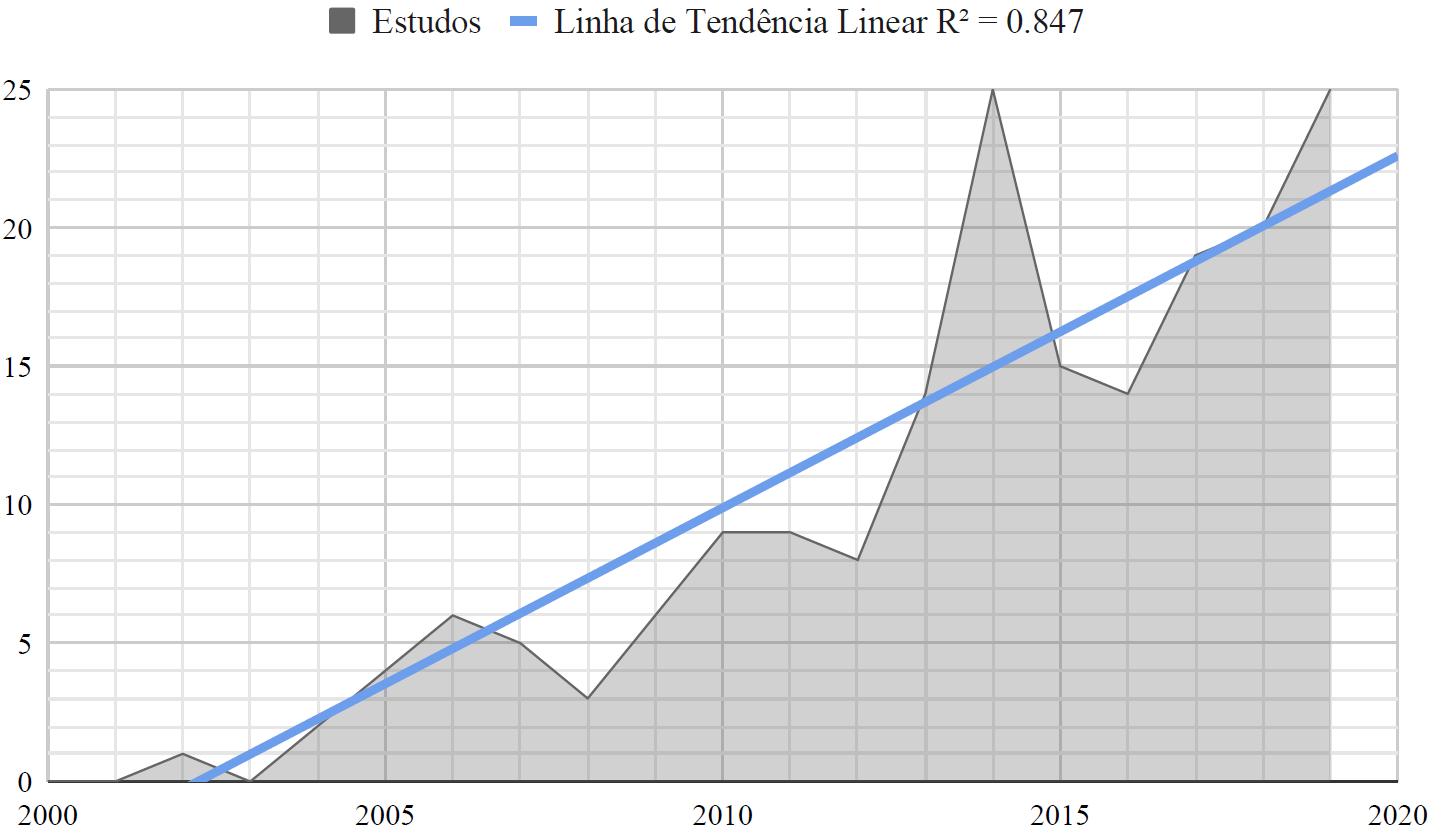
\includegraphics[width=.95\textwidth]{images/chapter2-sm-publications-timeline.png}
\fautor
\end{figure}

\simbolo{R^2}{Linha de Tendência Linear}

No que diz respeito às conferências, periódicos e fontes das publicações, esses dados também podem compor um racional interessante para futuras replicações. Sendo assim, todos os estudos primários deste MS foram ordenados pela quantidade de estudos selecionados (\autoref{results:table:publication-venues}). No contexto internacional, a presença de eventos identificados durante as buscas manuais (em \textbf{\textit{destaque}} na \autoref{results:table:publication-venues}) sugere uma execução efetiva dessa fase considerando o protocolo de busca adotado.

\begin{table}[htb]
\caption{Conferências/Periódicos mais relevantes.}
\label{results:table:publication-venues}
\centering
\begin{tabular}{lcc|lcc} \hline
\multicolumn{3}{c|}{\textbf{Internacionais (\textit{INT})}} & \multicolumn{3}{c}{\textbf{Nacionais (\textit{BRA})}} \\ \hline
\textbf{Nome} & \textbf{Fonte} & \textbf{Estudos} & \textbf{Nome} & \textbf{Fonte} & \textbf{Estudos} \\ \hline
\textit{\textbf{HCI International}} & \textit{\textbf{Springer}} & \textit{\textbf{12}} & RENOTE & CINTED & 13 \\ 
ICCHP & Springer & 8 & SBIE & CEIE & 13 \\ 
\textit{\textbf{ICALT}} & \textit{\textbf{IEEE}} & \textit{\textbf{6}} & WCBIE & CEIE & 11 \\ 
ASSETS & ACM & 6 & WIE & CEIE & 7 \\ 
\textit{\textbf{Computers \& Education}} & \textit{\textbf{Elsevier}} & \textit{\textbf{5}} & RBIE & CEIE & 2 \\ 
Procedia Computer Science & Elsevier & 5 & - & - & - \\ 
Outros & - & 97 & - & - & - \\ \hline
\multicolumn{2}{l}{\textbf{Total}} & \textbf{139} & \multicolumn{2}{l}{\textbf{Total}} & \textbf{46} \\ \hline
\end{tabular}
\end{table}

A seguir são discutidos os principais resultados deste estudo, de modo a responder cada QP definida no escopo do MS. Adicionalmente, com o objetivo de organizar os estudos primários, eles foram classificados com relação à sua origem: Internacional (\textit{INT})\footnote{Formulário de extração de dados Internacionais (INT): \url{https://bit.ly/SM-DataExtraction-INT}} ou Nacional (\textit{BRA})\footnote{Formulário de extração de dados Nacionais (BRA): \url{https://bit.ly/SM-DataExtraction-BRA}}. Com isso, os resultados podem ser analisados de forma isolada, o que facilita o planejamento e a condução de trabalhos futuros.

\subsubsection{QP1: Quais soluções tecnológicas vêm sendo propostas no processo de ensino-aprendizagem com línguas de sinais?}

As áreas presentes na \autoref{results:table:se-areas} destacam a importância intrínseca das arquiteturas de software na construção de TAs para línguas de sinais. Embora haja uma concentração significativa nas etapas de ``Construção'' e ``Projeto'', poucas soluções se mostraram realmente replicáveis ou adaptáveis a diferentes contextos educacionais, principalmente pela falta de detalhes técnicos.

\begin{table}[htb]
\caption{QP1: Áreas da ES no SWEBOK \cite{Bourque2014}.}
\label{results:table:se-areas}
\centering
\begin{tabular}{lcc|cc} \hline
 & \multicolumn{2}{c|}{\textit{\textbf{INT}}} & \multicolumn{2}{c}{\textit{\textbf{BRA}}} \\ \cline{2-5} 
\textbf{Área da ES} & \textbf{Estudos} & \textbf{\%} & \textbf{Estudos} & \textbf{\%} \\ \hline
Construção de Software & 65 & 47\% & 23 & 50\% \\
Projeto de Software & 47 & 34\% & 5 & 11\% \\
Fundamentos da Engenharia & 24 & 17\% & 9 & 19\% \\
Qualidade de Software & 3 & 2\% & 9 & 19\% \\ \hline
\textbf{Total} & \textbf{139} & \textbf{100\%} & \textbf{46} & \textbf{100\%} \\ \hline
\end{tabular}
\end{table}

Tecnicamente, a grande maioria das soluções é baseada em plataformas Web, Mobile ou Desktop, evidenciando uma preocupação genuína em criar TAs para diferentes plataformas de ensino-aprendizagem. No entanto, poucos estudos foram estruturados de forma a facilitar o seu reuso e extensibilidade. Além disso, menos da metade dos estudos apresentou avaliações empíricas formais, como \textit{Surveys}, Experimentos e Estudos de Caso, indicando uma falta de rigor científico em parte das pesquisas \cite{Pressman2016, Sommerville2015}.

Em contrapartida, avatares de línguas de sinais baseados em texto, como o \textit{Hand Talk}\footnote{Mais informações em \url{https://handtalk.me}} e o \textit{VLibras}\footnote{Mais informações em \url{https://gov.br/governodigital/pt-br/vlibras}}, destacam-se ao transformar texto em língua de sinais, evidenciando o potencial de TAs bem arquitetadas para potencializar a acessibilidade de conteúdos em diversos contextos educacionais. Portanto, a discussão sobre Arquiteturas de Software na \autoref{section:foundation:arch} será fundamental para compreender como essas soluções podem ser aprimoradas para desenvolver TAs verdadeiramente escaláveis.

\subsubsection{QP2: Quais tópicos educacionais são abordados?}

A \autoref{results:table:educational-topics} apresenta uma ampla diversidade de tópicos educacionais tendo em vista os OAs analisados, evidenciando o uso de TAs para línguas de sinais em diversos contextos. O que representa um esforço consciente em abordar diferentes temas no processo de ensino-aprendizagem, promovendo uma acessibilidade digital mais ampla e personalizada. 

\begin{table}[htb]
\caption{QP2: Tópicos Educacionais.}
\label{results:table:educational-topics}
\centering
\begin{tabular}{lcc|cc} \hline
 & \multicolumn{2}{c|}{\textit{\textbf{INT}}} & \multicolumn{2}{c}{\textit{\textbf{BRA}}} \\ \cline{2-5} 
\textbf{Tópico Educacional} & \textbf{Estudos} & \textbf{\%} & \textbf{Estudos} & \textbf{\%} \\ \hline
Línguas de Sinais & 59 & 42,5\% & 19 & 41,3\% \\
Geral & 48 & 34,5\% & 10 & 21,7\% \\
Língua de Sinais Escrita & 10 & 7,2\% & 3 & 6,5\% \\
Matemática & 7 & 5,0\% & - & - \\
Alfabeto & 6 & 4,3\% & 1 & 2,2\% \\
Ciência da Computação & 4 & 2,9\% & 4 & 8,7\% \\
Língua Falada do País & 2 & 1,4\% & 9 & 19,6\% \\
Outros & 3 & 2,2\% & - & - \\ \hline
\textbf{Total} & \textbf{139} & \textbf{100\%} & \textbf{46} & \textbf{100\%} \\ \hline
\end{tabular}
\end{table}

Com uma vasta gama de OAs inclusivos e adaptáveis, os educadores podem proporcionar experiências de aprendizado mais imersivas e eficazes, garantindo oportunidades igualitárias de desenvolvimento para todos os alunos, independentemente de suas habilidades ou desafios individuais. Tais resultados estabelecem a base para uma discussão mais aprofundada sobre OAs na \autoref{section:foundation:lo}, onde exploraremos como esses recursos podem ser projetados para atender demandas educacionais diversas.

\subsubsection{QP3: Quais línguas de sinais são abordadas?}

\sigla*{IAGen}{Inteligências Artificiais Generativas}

As línguas de sinais mais comuns, destacadas na \autoref{results:table:sign-languages}, juntamente com o crescente interesse em ASR multilíngue, abrem caminho para avanços significativos na acessibilidade. A capacidade das IAs Generativas (IAGen) de transcrever e traduzir fala em texto em múltiplas línguas viabiliza a integração de avatares de línguas de sinais baseados em texto, resultando em OAs mais inclusivos e versáteis.

\begin{table}[htb]
\caption{QP3: Línguas de Sinais.}
\label{results:table:sign-languages}
\centering
\begin{tabular}{lcc|cc} \hline
 & \multicolumn{2}{c|}{\textit{\textbf{INT}}} & \multicolumn{2}{c}{\textit{\textbf{BRA}}} \\ \cline{2-5} 
\textbf{Língua de Sinais} & \textbf{Estudos} & \textbf{\%} & \textbf{Estudo} & \textbf{\%} \\ \hline
ASL & 21 & 15.11\% & - & - \\
Libras & 16 & 11.51\% & 44 & 95.65\% \\
Geral & 15 & 10.79\% & - & - \\
SignWriting & 10 & 7.19\% & 2 & 4.35\% \\
ArSL & 10 & 7.19\% & - & - \\
PSL & 6 & 4.32\% & - & - \\
BSL & 6 & 4.32\% & - & - \\
MySL & 6 & 4.32\% & - & - \\
ISL & 5 & 3.60\% & - & - \\
Outras & 44 & 31.65\% & - & - \\ \hline
\textbf{Total} & \textbf{139} & \textbf{100\%} & \textbf{46} & \textbf{100\%} \\ \hline
\end{tabular}
\end{table}

Nesse cenário, línguas de sinais como a \textit{American Sign Language} (ASL) e a Libras, além de sistemas de escrita como o \textit{SignWriting}, podem se beneficiar dessas tecnologias, ampliando o acesso a conteúdos educacionais antes restritos aos formatos de áudio e vídeo. Esses resultados ressaltam a importância do ASR, que será aprofundado na \autoref{section:foundation:asr}.

A análise dos resultados obtidos pelas QP fornece um panorama do uso das TICs no ensino e aprendizado com línguas de sinais, revelando tanto lacunas quanto oportunidades para avanços significativos na criação de TAs ainda mais robustas. Essas descobertas abrem caminho para uma exploração detalhada de temas cruciais, como Arquiteturas de Software (\autoref{section:foundation:arch}), OAs (\autoref{section:foundation:lo}) e ASR (\autoref{section:foundation:asr}). Cada seção subsequente destaca como suas temáticas podem ajudar a superar os desafios identificados e a capitalizar nas oportunidades emergentes, contribuindo para um processo de ensino-aprendizagem mais inclusivo e acessível.

\section{Arquiteturas de Software: Bases Sólidas para Tecnologias Assistivas}
\label{section:foundation:arch}

Uma das principais lacunas identificadas no MS foi a carência de padrões e boas práticas que permitam o reuso e a adaptação das soluções no ensino e aprendizagem com línguas de sinais. Muitos dos estudos primários apresentaram contribuições técnicas relevantes, mas não detalharam as arquiteturas de software utilizadas, dificultando a evolução e derivação dessas soluções para outros contextos e domínios de aplicação. Por isso, discutiremos como as arquiteturas podem contribuir para o desenvolvimento de TAs replicáveis, flexíveis e independentes de tecnologia, seguindo alguns princípios e diretrizes da ES.

Nesse sentido, uma arquitetura de software pode ser definida como o conjunto de estruturas necessárias para o entendimento de um sistema, compreendendo desde seus componentes de software e hardware até suas relações/propriedades internas e externas \cite{Bass2021}. Essa definição enfatiza que a arquitetura não se limita apenas a decisões iniciais, mas inclui todas as decisões que moldam a estrutura do projeto e suas interações. A arquitetura é fundamental para a criação de sistemas complexos e facilita a análise de requisitos não funcionais, como desempenho, segurança e escalabilidade \cite{Pressman2016, Sommerville2015}.

Diferentemente de outras definições focadas em decisões antecipadas, a arquitetura, conforme \citeonline{Bass2021}, é sobre estruturas que permitem o raciocínio e a análise do sistema. Essa perspectiva permite uma compreensão mais ampla e flexível da arquitetura, considerando suas múltiplas dimensões e aspectos envolvidos no desenvolvimento e manutenção do software.

\subsection{Estruturas e Visões Arquiteturais}

Resumidamente, a arquitetura pode ser vista como um conjunto de estruturas que proporcionam diferentes perspectivas sobre o sistema, cada uma com seu foco específico, o qual pode ser necessário em diferentes fases do ciclo de vida do software. Formalmente, \citeonline{Bass2021} identificam três tipos principais de estruturas arquiteturais, que formam as principais visões neste contexto:

\begin{itemize}

    \item \textbf{Estruturas de Componentes e Conectores (C\&C)}: Estas estruturas focam nas interações em tempo de execução entre os componentes que realizam as funções do sistema. Componentes, que podem ser serviços, clientes, servidores ou filtros, são as unidades principais de computação. Os conectores, por sua vez, são os veículos de comunicação entre esses componentes, facilitando a troca de dados e a sincronização de processos. As estruturas C\&C são cruciais para entender o comportamento em tempo de execução, incluindo a interação entre componentes, a replicação de partes do sistema e a paralelização de tarefas \cite{Bass2021};
    
    \item \textbf{Estruturas de Módulos}: Estas estruturas particionam o sistema em unidades de implementação, conhecidas como módulos, que são responsáveis por funções específicas e são a base para a organização do trabalho de desenvolvimento. Módulos podem representar classes, pacotes ou divisões de funcionalidade, cada um com um papel definido no sistema. As relações entre os módulos, como uso, generalização e composição, ajudam a entender a estrutura estática do sistema e a gerenciar sua evolução e manutenção \cite{Bass2021};
    
    \item \textbf{Estruturas de Alocação}: Estas estruturas estabelecem a correspondência entre as estruturas de software e os componentes não software do sistema, como ambientes de desenvolvimento e execução. Elas respondem a questões críticas sobre onde cada elemento de software será executado, como os elementos estão armazenados e como são atribuídos às equipes de desenvolvimento. As estruturas de alocação são essenciais para a compreensão da distribuição do software e para a gestão de recursos durante todo o ciclo de vida do sistema \cite{Bass2021}.
    
\end{itemize}

Essas estruturas arquiteturais são análogas às diferentes especialidades médicas que focam em partes específicas do corpo humano, como ilustra a \autoref{chapter2:figure:physiological-structures}. Essa analogia facilita a compreensão de como diferentes visões se complementam para fornecer uma compreensão abrangente do sistema como um todo \cite{Bass2021}.

\begin{figure}[htb]
\centering
\caption{Fisiologia Humana: Análoga às Estruturas e Visões Arquiteturais}
\label{chapter2:figure:physiological-structures}
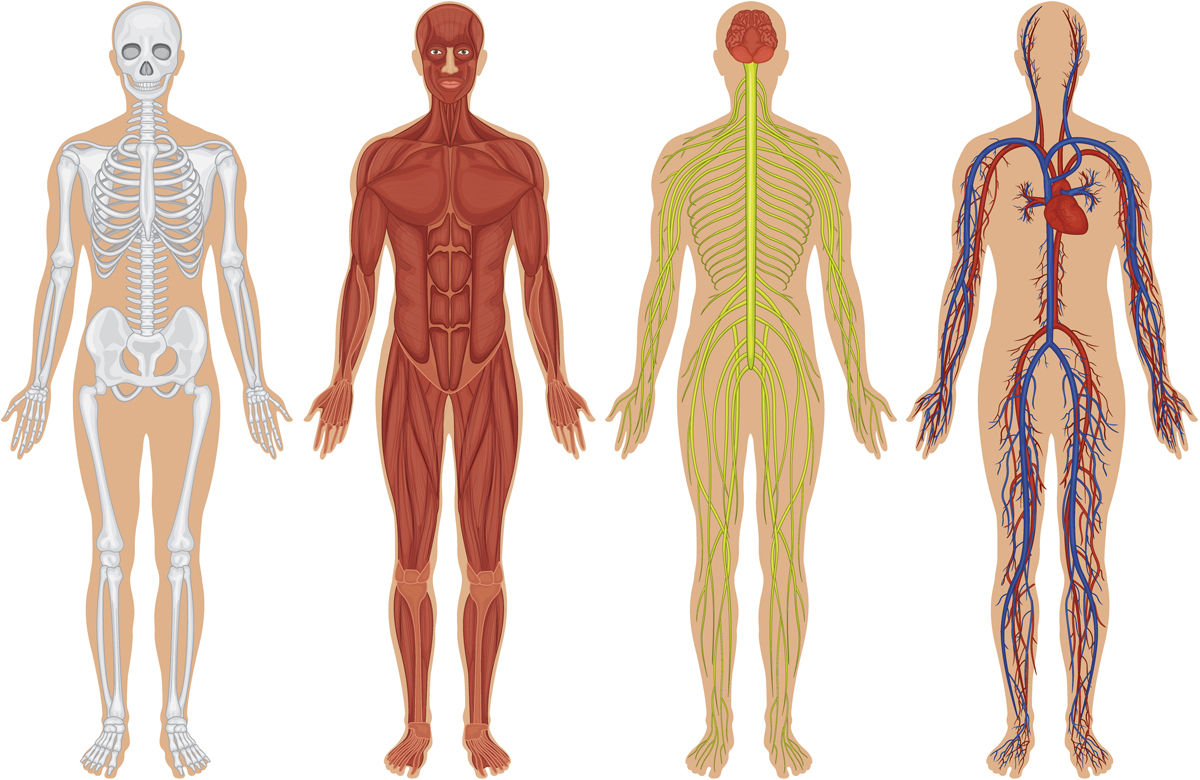
\includegraphics[width=0.60\textwidth]{images/chapter2-arch-physiological-structures.jpeg}
\end{figure}

Essas três categorias de estruturas facilitam a criação de representações visuais que auxiliam na compreensão da arquitetura de software em diferentes etapas do desenvolvimento. A arquitetura \textit{Speech2Learning}, por exemplo, adota essas estruturas para garantir clareza arquitetural desde sua concepção até a avaliação em seus estudos de caso (detalhes nos Capítulos \ref{chapter3} e \ref{chapter4}). Essa abordagem sistematiza e torna mais eficiente a implementação de TAs.

\subsection{O que Torna uma Arquitetura ``Boa''?}

Na prática, a arquitetura de software é uma abstração que destaca detalhes relevantes para a compreensão e análise do sistema, omitindo informações desnecessárias para o raciocínio sobre ele. A abstração é crucial para gerir a complexidade, permitindo que arquitetos e desenvolvedores se concentrem em aspectos essenciais sem se preocuparem com detalhes de implementação. A arquitetura trata dos elementos públicos do sistema, ou seja, aqueles que interagem entre si através de interfaces, enquanto os detalhes privados de implementação não são considerados \cite{Bass2021}.

Padrões arquiteturais são composições de elementos arquiteturais que foram documentadas e disseminadas devido à sua eficácia em resolver problemas recorrentes em diferentes domínios. Esses padrões fornecem abordagens comprovadas para o design de sistemas e são fundamentais para alcançar os atributos de qualidade desejados, como modularidade e facilidade de manutenção \cite{Bass2021}. Por exemplo, o padrão de arquitetura em camadas é amplamente utilizado para sistemas que necessitam de alta modularidade, enquanto o padrão de microsserviços é ideal para sistemas que requerem escalabilidade e resiliência \cite{Pressman2016, Sommerville2015}.

Entretanto, não existe uma arquitetura intrinsecamente ``boa'' ou ``ruim''; a adequação de uma arquitetura depende de como ela atende aos requisitos específicos do sistema. Uma arquitetura projetada para um sistema de comércio eletrônico pode não ser adequada para um sistema de controle de voo, por exemplo. A avaliação da arquitetura em relação a objetivos específicos é crucial para garantir que ela atenda às necessidades do sistema \cite{Pressman2016, Sommerville2015}.

Para orientar o desenvolvimento de uma boa arquitetura de software, \citeonline{Bass2021} propõem algumas boas práticas, categorizadas em recomendações de processo e estruturais. Primeiramente, as \textbf{recomendações de processo} focam na maneira como a arquitetura deve ser desenvolvida e gerenciada ao longo do ciclo de vida do sistema, garantindo que a integridade conceitual e a qualidade sejam mantidas de forma contínua:

\begin{enumerate}
    \item \textbf{Desenvolvimento por lideranças técnicas}: É fundamental que a arquitetura seja concebida por um arquiteto ou uma pequena equipe de arquitetos com um líder técnico identificado, garantindo a integridade conceitual e a consistência técnica. Esse princípio também se aplica a projetos ágeis e de código aberto, evitando designs impraticáveis e desconectados da realidade do desenvolvimento.
    
    \item \textbf{Foco nos requisitos de qualidade}: A arquitetura deve se basear continuamente em uma lista priorizada de requisitos de qualidade bem definidos. Esses requisitos informam as decisões de \textit{trade-offs} que sempre ocorrem, sendo mais relevantes do que a funcionalidade em si.
    
    \item \textbf{Documentação por meio de visões arquiteturais}: A arquitetura deve ser documentada através de visões que representem uma ou mais estruturas arquiteturais. Essas visões devem abordar as preocupações dos \textit{stakeholders} mais importantes e apoiar o cronograma do projeto, fornecendo uma documentação que pode ser inicialmente minimalista, mas detalhada posteriormente.
    
    \item \textbf{Avaliação contínua dos atributos de qualidade}: A arquitetura deve ser avaliada quanto à sua capacidade de fornecer os principais atributos de qualidade do sistema. Isso deve ocorrer no início do ciclo de vida, proporcionando os maiores benefícios, e ser repetido conforme necessário para garantir que alterações na arquitetura ou no ambiente não tornem o design obsoleto.
    
    \item \textbf{Implementação incremental e adaptativa}: A arquitetura deve permitir a implementação incremental, evitando a integração total de uma só vez, o que raramente funciona. Isso pode ser alcançado através da criação de um sistema esquelético, no qual os caminhos de comunicação são exercidos inicialmente com funcionalidade mínima, permitindo o crescimento incremental do sistema e a refatoração conforme necessário.
\end{enumerate}

Por sua vez, as \textbf{recomendações estruturais} dizem respeito à organização interna da arquitetura, enfatizando a importância da modularidade, da separação de responsabilidades e da flexibilidade na integração dos componentes, visando a criação de um sistema robusto e facilmente evolutivo:

\begin{enumerate}
    \item \textbf{Modularização e separação de preocupações}: A arquitetura deve apresentar módulos bem definidos, cujas responsabilidades funcionais são atribuídas com base nos princípios de ocultação de informações e separação de preocupações. Esses módulos devem encapsular aspectos passíveis de mudança, isolando o software dos efeitos dessas mudanças.
    
    \item \textbf{Uso de padrões arquiteturais bem estabelecidos}: A arquitetura deve alcançar atributos de qualidade usando padrões arquiteturais e táticas bem estabelecidos e específicos para cada atributo. Isso proporciona uma base sólida para o design, garantindo que os requisitos de qualidade sejam atendidos de maneira eficaz.
    
    \item \textbf{Flexibilidade em relação a versões de produtos}: A arquitetura nunca deve depender de uma versão específica de um produto comercial ou ferramenta. Se isso for inevitável, deve ser estruturada de forma que a mudança para uma versão diferente seja simples e barata.
    
    \item \textbf{Separação entre componentes produtores e consumidores de dados}: Os módulos que produzem dados devem ser separados dos módulos que consomem esses dados. Isso aumenta a manutenibilidade, permitindo que mudanças sejam confinadas ao lado da produção ou do consumo de dados, facilitando atualizações incrementais.
    
    \item \textbf{Flexibilidade na correspondência entre módulos e componentes}: Não se deve esperar uma correspondência um-para-um entre módulos e componentes. Em sistemas com concorrência, por exemplo, múltiplas instâncias de um componente podem ser executadas em paralelo, cada uma construída a partir do mesmo módulo.
    
    \item \textbf{Alocação flexível de processos}: Projete cada processo para ser executado em qualquer processador, permitindo fácil realocação, inclusive durante a execução. Isso é essencial em ambientes de virtualização e nuvem, onde os recursos computacionais podem variar.
    
    \item \textbf{Consistência e simplicidade nos padrões de interação}: A arquitetura deve conter um pequeno número de padrões simples de interação entre componentes. O sistema deve realizar as mesmas funções da mesma maneira em todas as partes, o que facilita a compreensão, reduz o tempo de desenvolvimento, além de aumentar confiabilidade e manutenibilidade.
    
    \item \textbf{Gestão eficaz de áreas de contenção de recursos}: A arquitetura deve conter um conjunto específico e pequeno de áreas de contenção de recursos, cuja resolução deve ser claramente especificada e mantida. Por exemplo, se a utilização da rede é uma preocupação, o arquiteto deve produzir diretrizes para cada equipe de desenvolvimento que resultem em níveis aceitáveis de tráfego de rede.
\end{enumerate}

Em suma, uma arquitetura de software bem projetada não só atende aos requisitos funcionais imediatos, mas também oferece uma base sólida que permite a evolução e adaptação contínua do sistema, especialmente em áreas críticas como a educação inclusiva. A flexibilidade da arquitetura é essencial para suportar a evolução contínua das TICs e a adaptação às necessidades dos aprendizes, garantindo que as soluções sejam sustentáveis e capazes de atender às necessidades dos alunos a longo prazo.

Nesse contexto, a arquitetura \textit{Speech2Learning} surge como uma proposta para impulsionar a construção de TAs. Projetada para integrar soluções de ASR, ela visa facilitar a criação de OAs mais acessíveis a uma ampla gama de aprendizes \cite{FalvoJr2023_HICSS}. Nos próximos capítulos, exploraremos em detalhes os conceitos de OAs e ASR, aprofundando nosso entendimento sobre como essas tecnologias se entrelaçam e formam a base da \textit{Speech2Learning}.

\section{Objetos de Aprendizagem: Diversidade em Conteúdos Educacionais}
\label{section:foundation:lo}

A diversidade em conteúdos educacionais é uma necessidade cada vez mais reconhecida, como evidenciado em nosso MS. Sendo assim, os OAs emergem como uma solução promissora para atender a essa demanda, permitindo a criação de recursos personalizados e adaptáveis a diferentes contextos e públicos. No âmbito da arquitetura \textit{Speech2Learning}, os OAs desempenham um papel fundamental no acesso a materiais didáticos audíveis, enriquecidos pela tecnologia de ASR para maior acessibilidade \cite{FalvoJr2023_HICSS}.

Os OAs abrangem um amplo espectro de recursos digitais projetados para enriquecer o processo de ensino-aprendizagem. Eles vão além da mera entrega de conteúdo, proporcionando uma experiência mais rica e interativa \cite{Wiley2000}. A importância da multimídia no aprendizado é destacada por \citeonline{Mayer2021}, que argumenta que a combinação eficaz de texto, áudio, vídeo e elementos interativos pode potencializar a retenção e aplicação do conhecimento.

\sigla*{IEEE}{\textit{Institute of Electrical and Electronics Engineers}}

O \citeonline{LOM2000} define os OAs como entidades, digitais ou não-digitais, que podem ser usadas, reutilizadas ou referenciadas durante o ensino com suporte tecnológico. Essa definição abrange uma vasta gama de recursos, incluindo conteúdos multimídia, software instrucional, eventos educacionais, entre outros. \citeonline{Wiley2000} simplifica essa concepção ao descrever os OAs como recursos digitais que podem ser reutilizados para facilitar a aprendizagem, destacando a adaptabilidade e a reusabilidade como características centrais dos OAs.

A essência dos OAs reside na criação de pequenos módulos instrucionais reutilizáveis, combináveis de diferentes maneiras para atender às necessidades específicas de aprendizagem. Essa abordagem permite que educadores personalizem o ensino, adaptando materiais didáticos às suas metas pedagógicas individuais. O resultado é um processo de ensino-aprendizagem mais dinâmico, onde diferentes recursos se conectam para formar um todo coeso (\autoref{chapter2:figure:lo-mindmap}).

\begin{figure}[htb]
\centering
\caption{Mapa Conceitual Sobre Objetos de Aprendizagem}
\label{chapter2:figure:lo-mindmap}
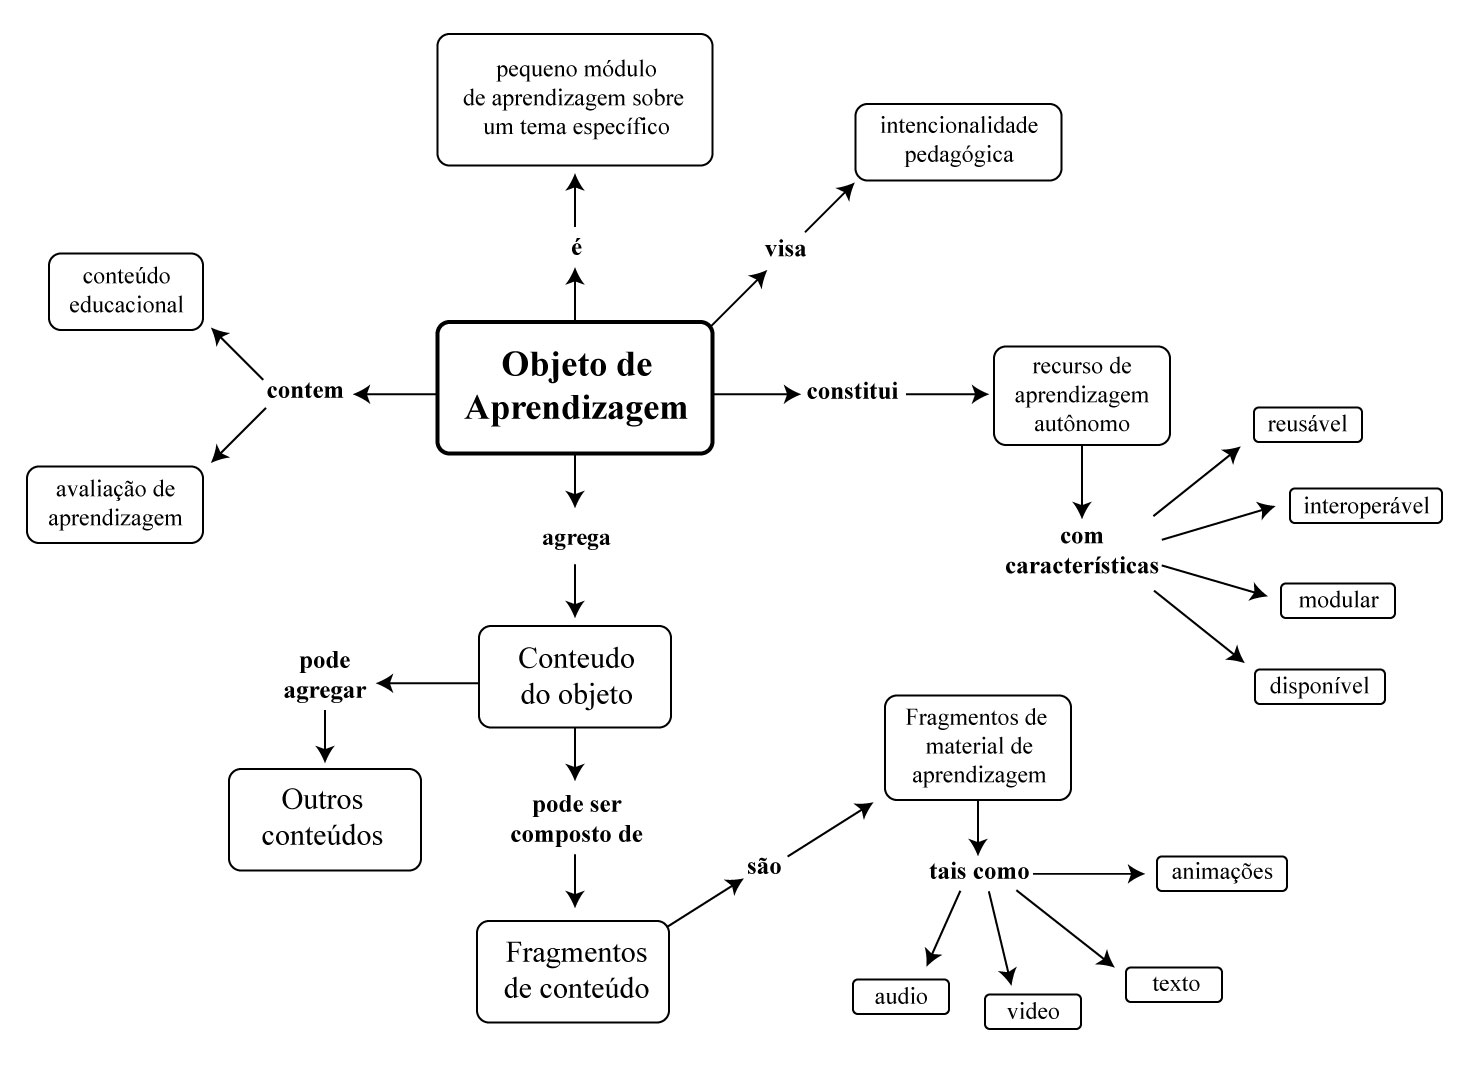
\includegraphics[width=0.8\textwidth]{images/chapter2-lo-mindmap.jpg}
\fadaptada{Tarouco2021}
\end{figure}

\subsection{Estratégias de Identificação e Utilização de OAs}

O uso e reuso de OAs envolve várias estratégias que facilitam sua adaptação a diferentes contextos educacionais. Conforme discutido por \citeonline{Tarouco2021}, os OAs podem variar em tamanho, escopo e nível de granularidade, afetando diretamente sua reusabilidade (\autoref{chapter2:figure:lo-granularity}). Objetos com granularidade alta, como imagens ou pequenos vídeos, são mais fáceis de reutilizar devido à sua simplicidade e especificidade. Em contraste, OAs de granularidade baixa, como cursos, oferecem uma experiência educacional mais completa e integrada, mas são mais difíceis de adaptar a novos contextos de ensino-aprendizagem.

\begin{figure}[htb]
\centering
\caption{Granularidade de Objetos de Aprendizagem}
\label{chapter2:figure:lo-granularity}
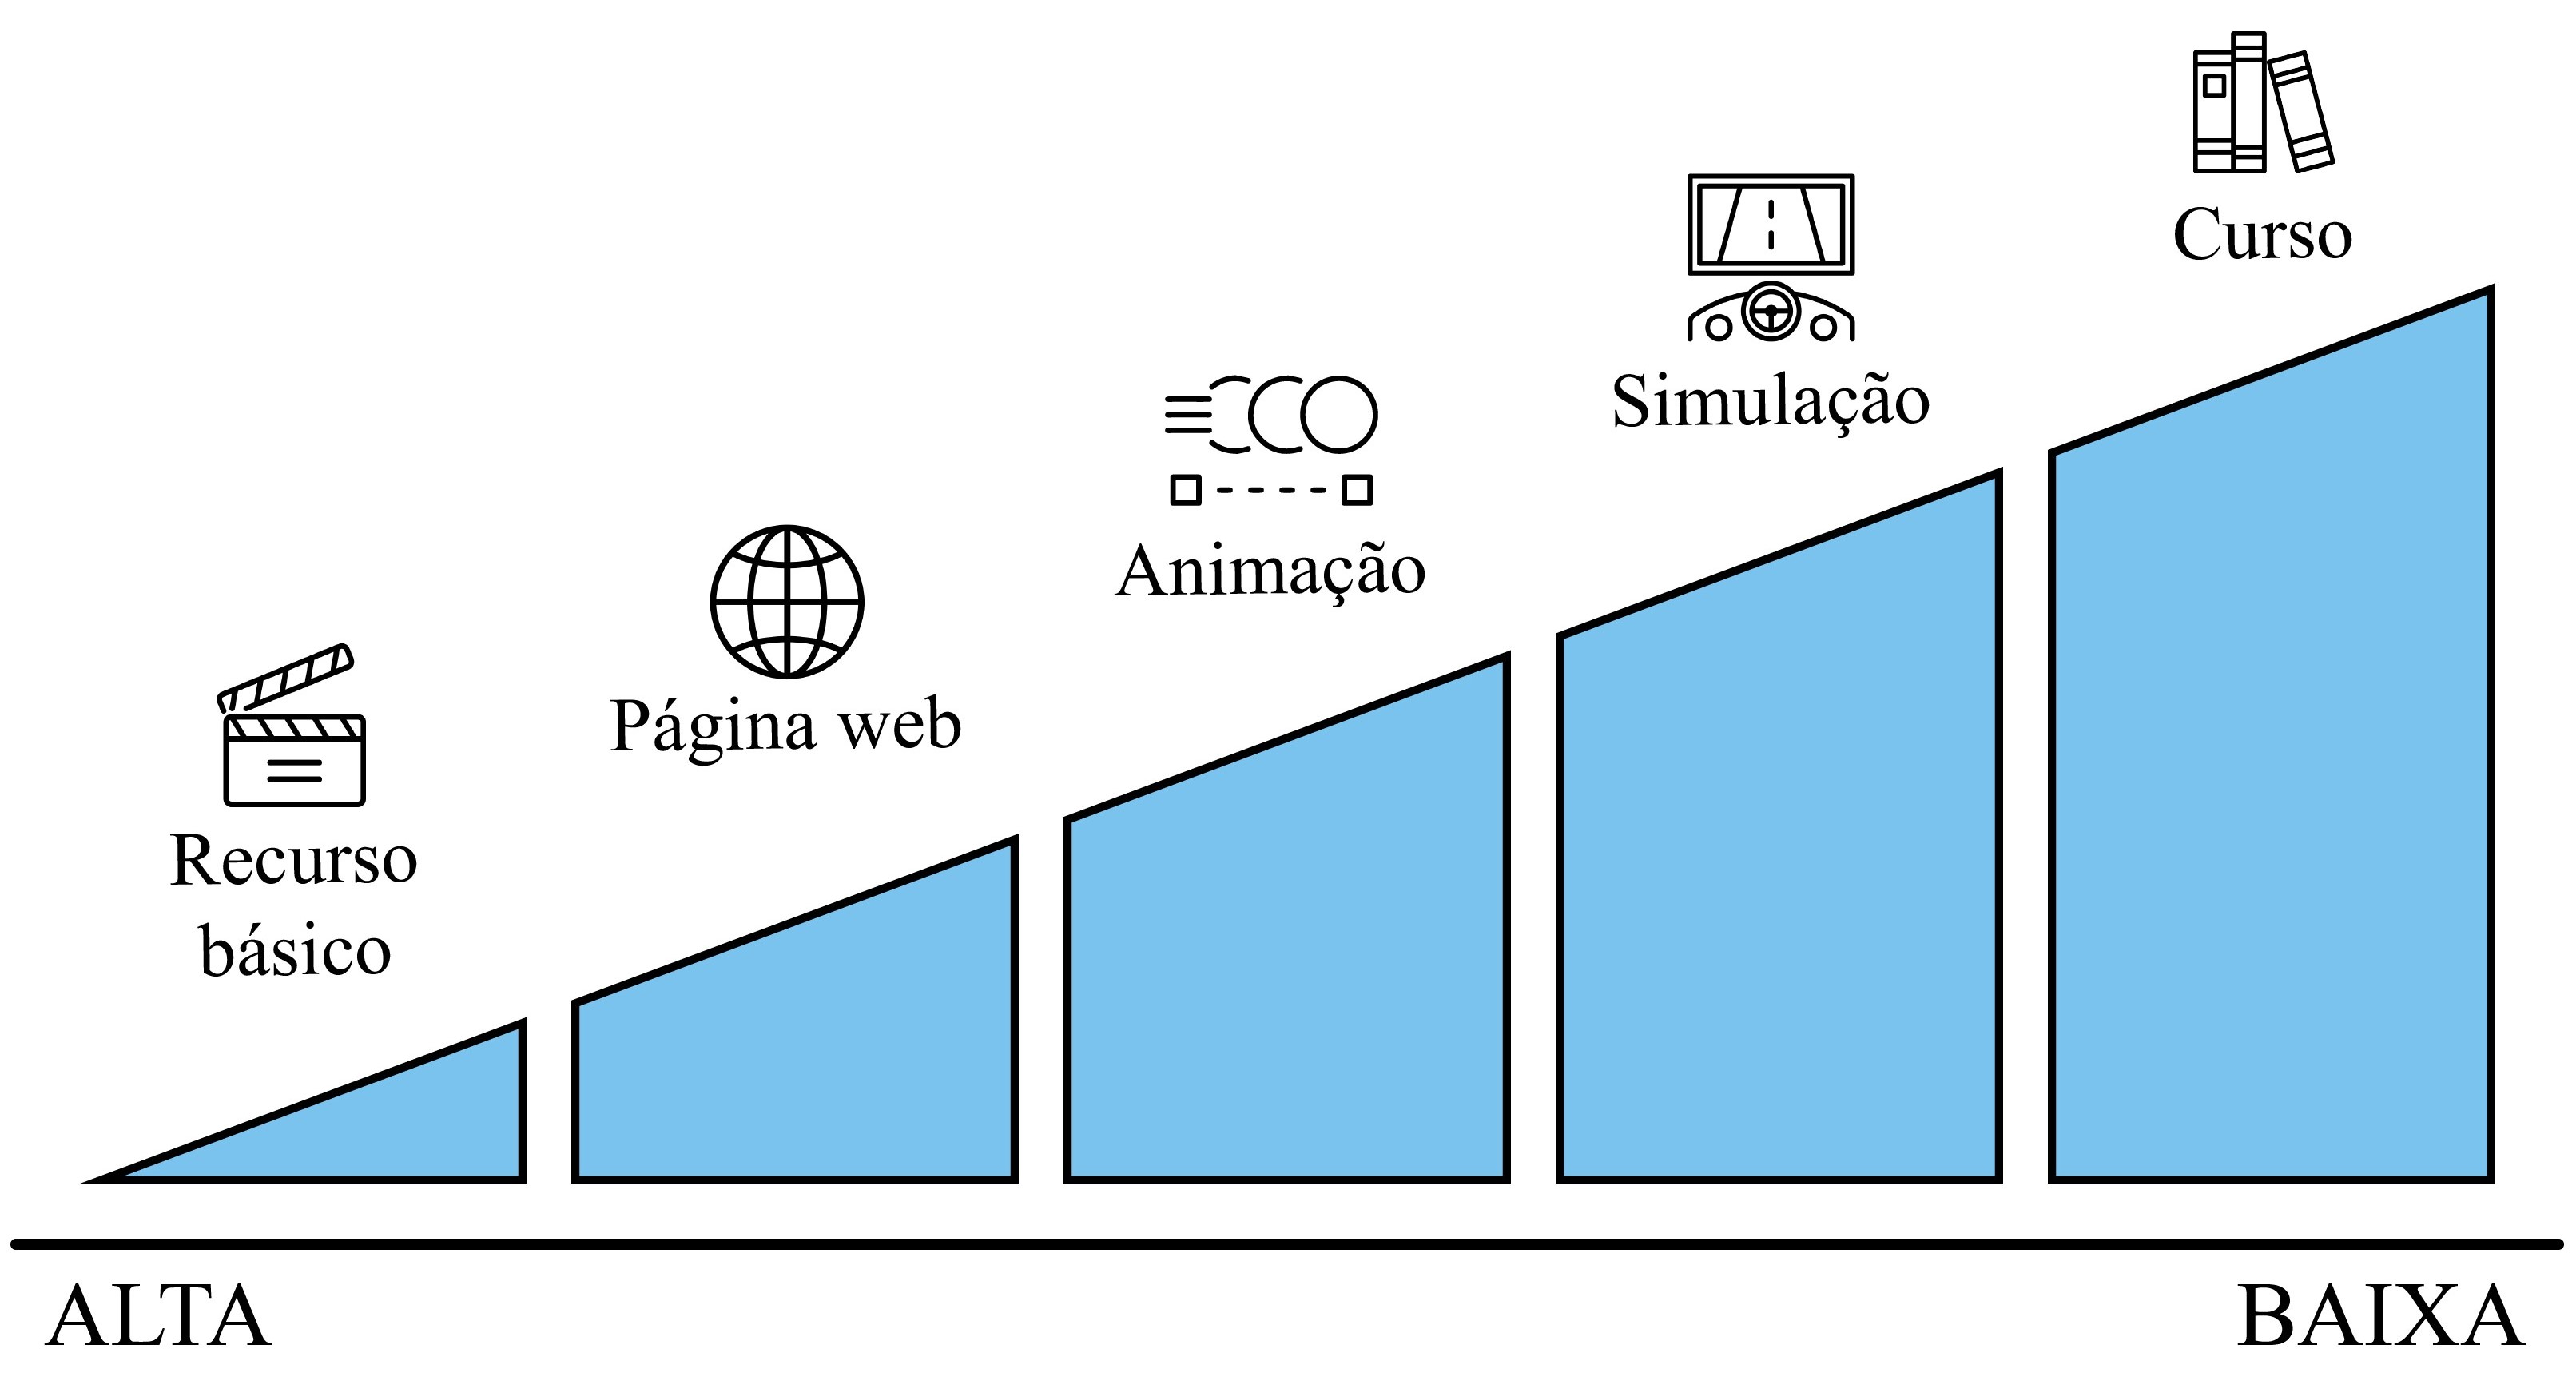
\includegraphics[width=0.65\textwidth]{images/chapter2-lo-granularity.jpg}
\fadaptada{Tarouco2021}
\end{figure}

A granularidade dos OAs está intimamente ligada à intencionalidade pedagógica, definida pela finalidade educacional para a qual o objeto foi criado. De acordo com \citeonline{Bloom1984}, a eficácia de um OA depende da clareza de seus objetivos pedagógicos e da adequação às necessidades dos estudantes. Dessa forma, a escolha de OAs deve considerar tanto a granularidade quanto a intencionalidade pedagógica para garantir uma aprendizagem eficaz e significativa.

Nesse sentido, a adoção de padrões de metadados é essencial para a organização, indexação e reutilização de OAs. \citeonline{Santana2023} destacam a importância desses padrões e sua aplicabilidade no contexto da ES experimental, cujo compartilhamento de OAs é vital para replicações e pesquisas futuras. A \autoref{chapter2:table:lo-metadata} apresenta uma comparação entre vários padrões de metadados, destacando suas características principais:

\begin{itemize}
    \item \textit{Dublin Core}\footnote{Mais informações em \url{https://dublincore.org}}: Um padrão internacional que fornece um conjunto simples e padronizado de termos para descrever recursos. O Dublin Core é conhecido por sua simplicidade e extensibilidade, permitindo sua aplicação em diversos contextos, desde bibliotecas digitais até sistemas de informação corporativos.
    \item \sigla{SCORM}{\textit{Sharable Content Object Reference Model}}\footnote{Mais informações em \url{https://adlnet.gov/scorm}}: Um conjunto de padrões e especificações para e-learning que define a comunicação entre o conteúdo de aprendizado online e os sistemas de gerenciamento de aprendizado (LMS). Desenvolvido pela Advanced Distributed Learning (ADL), o SCORM facilita a interoperabilidade e a reutilização de conteúdos educacionais em diferentes plataformas de aprendizado.
    \item \textit{Motion Imagery Standard Board} (MISB)\footnote{Mais informações em \url{https://nsgreg.nga.mil/misb.jsp}}: Padrão desenvolvido para a gestão e utilização de imagens em movimento, particularmente em contextos que exigem alta precisão e interoperabilidade, como vigilância e análise de vídeo. O MISB, parte da National Geospatial-Intelligence Agency (NGA), assegura que os dados de vídeo sejam consistentes e compatíveis em diferentes sistemas.
    \item \sigla{LOM}{\textit{Learning Object Metadata}}\footnote{Mais informações em \url{https://ieeexplore.ieee.org/document/9262118}}: Um padrão para a descrição de metadados de OAs, abrangendo aspectos como a finalidade educacional, estrutura, nível de agregação e condições de uso. Publicado pelo IEEE, o LOM é amplamente utilizado para descrever e categorizar recursos educacionais digitais, facilitando sua descoberta e reutilização.
    \item \sigla{RDF}{\textit{Resource Description Framework}}\footnote{Mais informações em \url{https://w3.org/rdf}}: Uma especificação da W3C que fornece uma base para a descrição de recursos da web. O RDF é utilizado para modelagem de informações, permitindo a interoperabilidade entre diferentes sistemas de informação e facilitando a integração de dados de diversas fontes.
\end{itemize}

\begin{table}[htb]
\caption{Comparação Entre os Padrões de Metadados} 
\label{chapter2:table:lo-metadata}
\begin{tabular}{P{3.5cm}|P{3cm}|P{3cm}|P{3cm}}\hline
\textbf{Padrão de Metadados} & \textbf{Documentação Completa} & \textbf{Processamento Automatizado} & \textbf{Flexibilidade para ES} \\ \hline
Dublin Core & X & X & X \\ 
SCORM & X & X & X \\
MISB & X & X & \\
LOM & X & X & X \\
RDF & X & X & X \\ \hline
\end{tabular}
\fadaptada{Santana2023}
\end{table}

Segundo \citeonline{Santana2023}, o Dublin Core se destaca por sua simplicidade, documentação abrangente e capacidade de processamento automatizado, permitindo sua aplicação em diferentes linhas de pesquisa na área da ES. No entanto, no contexto deste trabalho, qualquer padrão de metadados pode ser adequado, visto que o papel de uma arquitetura de software não é o de definir ``detalhes de implementação''. 

Por outro lado, o LOM merece destaque pelo seu foco intrínseco em aspectos educacionais, demonstrando uma sinergia natural com o conceito de OAs. Além disso, com exceção do MISB, todos os padrões são tão robustos quanto o Dublin Core, considerando os critérios de comparação da \autoref{chapter2:table:lo-metadata}.

Ao conhecer os conceitos de granularidade e padrões de metadados, fica mais simples entendermos como os OAs podem ser encontrados. Nesse sentido, os Repositórios de Objetos de Aprendizagem (ROAs) são plataformas que armazenam e disponibilizam OAs para educadores, estudantes e desenvolvedores. Eles desempenham um papel crucial na disseminação de recursos educacionais e na promoção do uso e reuso de OAs. No Brasil, de acordo com \citeonline{Tarouco2021}, alguns dos principais ROAs incluem: \textit{Portal do Professor}\footnote{Mais informações em \url{http://portaldoprofessor.mec.gov.br}}, \textit{Domínio Público}\footnote{Mais informações em \url{http://www.dominiopublico.gov.br}} e \textit{eduCAPES} \footnote{Mais informações em \url{https://educapes.capes.gov.br}}.

A utilização de padrões de metadados, como o LOM, nesses repositórios facilita a indexação e a busca eficiente de OAs, permitindo que educadores encontrem rapidamente os recursos que atendam às suas necessidades pedagógicas. A combinação de granularidade adequada e metadados padronizados assegura que os OAs possam ser reutilizados em diversos contextos educacionais, maximizando seu impacto e alcance.

%Um exemplo prático da adaptabilidade dos OAs é a inclusão de transcrições em materiais audíveis, como videoaulas. Essa prática não apenas flexibiliza o acesso à informação para todos os alunos, mas também destaca a capacidade dos OAs de se adaptarem às necessidades de uma gama diversificada de aprendizes, promovendo uma educação mais inclusiva. O potencial de adaptação dos OAs reforça a importância das TICs, como o ASR, na ampliação da acessibilidade e personalização dos conteúdos educacionais, conforme identificado no MS como um \textit{insight} relevante para a concepção da arquitetura \textit{Speech2Learning} \cite{FalvoJr2023_HICSS}.

A granularidade, os padrões de metadados e os repositórios de OAs convergem para apoiar a intencionalidade pedagógica. A intencionalidade pedagógica, por sua vez, refere-se à finalidade educacional para a qual os OAs são criados e utilizados. De acordo com \citeonline{Bloom1984}, a eficácia de um OA depende da clareza de seus objetivos pedagógicos e da adequação às necessidades dos estudantes.

A próxima seção discorrerá sobre a intencionalidade pedagógica, exemplificando como a Taxonomia de Bloom e sua revisão podem ser aplicadas na seleção e utilização de OAs para maximizar o processo de ensino-aprendizagem.

\subsection{Intencionalidade Pedagógica}

A intencionalidade pedagógica dos OAs pode ser exemplificada pela Taxonomia de Bloom, que categoriza objetivos educacionais em uma hierarquia de complexidade cognitiva \cite{Bloom1984}. Em um trabalho mais recente, \citeonline{Krathwohl2002} propôs uma revisão da taxonomia original, passando a trabalhar este sistema de classificação numa perspectiva bi-dimensional. A primeira é a dimensão do conhecimento e desdobra-se em quatro tipos: Factual, Conceitual, Procedimental e Metaconhecimento.

De acordo com \citeonline{Krathwohl2002}, a segunda dimensão trata sobre os processos cognitivos (comumente chamada de Taxonomia de Bloom Revisada), expressos através das seis categorias adaptadas da taxonomia original de \citeonline{Bloom1984}. O autor introduziu mudanças significativas, com destaque para o uso de verbos ativos em vez de substantivos e a reestruturação de alguns dos níveis. Como resultado, a nova versão organiza os objetivos de aprendizagem nas seguintes categorias: Recordar, Entender, Aplicar, Analisar, Avaliar e Criar \cite{Krathwohl2002}.

Poder usar um OA em diferentes contextos e por diversos usuários é uma de suas características fundamentais. Alguns OAs podem ser mais orientados a trabalhar o desenvolvimento de competências para alcançar uma ou outra categoria, mas podem-se encontrar objetos que são apropriados para mais de uma categoria, ou seja, eles podem ser utilizados em diversas etapas do processo de ensino-aprendizagem como:

\begin{itemize}
    \item \textbf{Etapa A}: Como introdução ao conteúdo a ser estudado;
    \item \textbf{Etapa B}: Para demonstração da teoria estudada;
    \item \textbf{Etapa C}: Como exemplo de aplicação do conteúdo estudado;
    \item \textbf{Etapa D}: Como instrumento de avaliação da aprendizagem.
\end{itemize}

%A \autoref{chapter2:lo:bloom-evolution} compara as categorias da taxonomia original e revisada, fornecendo descrições claras para cada nível \citeonline{Tarouco2021}.
% \begin{table}[htb]
% \centering
% \caption{Taxonomia Original \cite{Bloom1984} e Revisada \cite{Krathwohl2002}}
% \label{chapter2:lo:bloom-evolution}
% \begin{tabular}{C{2.4cm}|C{1.9cm}|p{10cm}} \hline
% \textbf{Original} & \textbf{Revisada} & \textbf{Descrição da Categoria} \\ \hline
% Conhecimento                & Recordar                    & Capacidade de reter conhecimento na memória de longo prazo.         \\ \hline
% Compreensão                 & Entender                    & Capacidade de construir significado a partir do material instrucional. \\ \hline
% Aplicação                   & Aplicar                     & Capacidade de utilizar o(s) procedimento(s) adequado(s) à situação vivenciada. \\ \hline
% Análise                     & Analisar                    & Capacidade de identificar diferentes partes constituintes de um material compreendendo suas inter-relações. \\ \hline
% Síntese                     & Avaliar                     & Capacidade de estabelecer julgamentos a partir de critérios e padrões. \\ \hline
% Avaliação                   & Criar                       & Capacidade de transpor o conhecimento construído para novas situações a partir de produtos originais de autoria do próprio estudante. \\ \hline
% \end{tabular}
% \fadaptada{Tarouco2021}
% \end{table}

Além disso, os OAs podem ser utilizados de forma individual ou coletiva. A escolha dependerá da intencionalidade pedagógica do professor e de sua escolha metodológica. A \autoref{chapter2:lo:samples-bloom-and-steps} ilustra exemplos de atividades com diferentes tipos de OAs, classificados de acordo com as duas dimensões propostas por \citeonline{Krathwohl2002} e apresentadas nesta ordem na Tabela: 1. Taxonomia de Bloom Revisada (Processo Cognitivo); 2. Etapas de Ensino-Aprendizagem.

\begin{table}[htbp]
\small
\centering
\caption{Tipos de OAs: Processos Cognitivos e Etapas de Ensino}
\label{chapter2:lo:samples-bloom-and-steps}
\begin{tabular}{lP{1.37cm}|P{1.35cm}|P{1.12cm}|P{1.3cm}|P{1.1cm}|P{0.9cm}*{4}{|P{0.4cm}}}
\hline
\multirow{2}{*}{\textbf{Tipo de OA}} & \multicolumn{6}{c|}{\textbf{Processo Cognitivo}} & \multicolumn{4}{c}{\textbf{Etapa de Ensino}} \\ \cline{2-11}
 & Recordar & Entender & Aplicar & Analisar & Avaliar & Criar & A & B & C & D \\ \hline
Texto & \faCheckCircle & \faCheckCircle & \faCheckCircle & \faCheckCircle & \faCheckCircle & \faCheckCircle & \faCheck & \faCheck & \faCheck & \faCheck \\
Jogo & \faCheckCircle & \faCheckCircle & \faCheckCircle & \faCheckCircleO & \faCheckCircleO & \faCheckCircleO & \faCheck & \faCheck & \faCheck & \faCheck \\
Simulação & \faCheckCircle & \faCheckCircle & \faCheckCircle & \faCheckCircleO & \faCheckCircleO & \faCheckCircleO & \faCheck & \faCheck & \faCheck & \faCheck \\
Áudio/Vídeo & \faCheckCircle & \faCheckCircle & \faCheckCircleO & \faCheckCircle & \faCheckCircleO & \faCheckCircleO & \faCheck & \faCheck & \faCheck & \faCheck \\
Slides & \faCheckCircle & \faCheckCircle & \faCheckCircleO & \faCheckCircle & \faCheckCircleO & \faCheckCircleO & \faCheck & \faCheck & \faCheck & \faCheck \\
Exercícios & \faCheckCircle & \faCheckCircle & \faCheckCircle & \faCheckCircle & \faCheckCircleO & \faCheckCircleO & \faCheck & \faTimes & \faTimes & \faCheck \\
Mapa Mental & \faCheckCircle & \faCheckCircle & \faCheckCircle & \faCheckCircle & \faCheckCircleO & \faCheckCircle & \faCheck & \faCheck & \faCheck & \faCheck \\
Experimento & \faCheckCircle & \faCheckCircle & \faCheckCircle & \faCheckCircle & \faCheckCircle & \faCheckCircleO & \faCheck & \faCheck & \faCheck & \faCheck \\
Infográfico & \faCheckCircle & \faCheckCircle & \faCheckCircle & \faCheckCircle & \faCheckCircle & \faCheckCircle & \faCheck & \faCheck & \faCheck & \faCheck \\ \hline
\end{tabular}
\fadaptada{Mayer2021}
\caption*{Legenda: \faCheckCircle~(uso comum); \faCheckCircleO~(uso em potencial); \faCheck~(aplicável); \faTimes~(não aplicável).}
\end{table}

Com isso, fica evidente a flexibilidade dos conteúdos do tipo texto no processo de ensino-aprendizagem, que são comumente usados em todos os itens da taxonomia, além de fazer parte de todas as etapas de ensino, demonstrando seu impacto na educação atualmente. Essa característica foi importante para definirmos o escopo da \textit{Speech2Learning} em tornar OAs audíveis mais acessíveis através de ASR, transformando conteúdos de áudio/vídeo em texto, aumentando assim o alcance e acessibilidade desse tipo de OAs.

\section{Reconhecimento de Fala: Promovendo Acessibilidade Digital com IA}
\label{section:foundation:asr}

Na era digital, a educação está em constante evolução à medida que as tecnologias emergentes podem remodelar as abordagens pedagógicas tradicionais. Neste contexto, o ASR, interpretado neste trabalho como um sinônimo de STT, emerge como uma ferramenta poderosa. O conceito de ASR não apenas pode potencializar a acessibilidade de conteúdos com transcrições e legendas, mas também representa um passo significativo em direção a uma educação mais inclusiva. Nesse sentido, concordamos com \citeonline{Homburg2019} sobre o potencial do ASR nas TAs para surdos, dentre as quais destacamos os avatares de línguas de sinais baseados em texto em nosso MS \cite{FalvoJr2020_FIE, FalvoJr2020_SBIE, FalvoJr2021_RENOTE}.

Segundo \citeonline{fleischmann2021}, a ascensão do ensino remoto, acelerada por circunstâncias como a pandemia da COVID-19, impulsionou a busca por métodos inovadores para a criação e compartilhamento de conteúdos educacionais. Nessa conjuntura, o ASR se consolidou como uma ferramenta promissora, particularmente em ambientes colaborativos ou conferências online. 

Desta forma, soluções baseadas em ASR desempenham um papel vital ao quebrar barreiras linguísticas, otimizando a comunicação entre falantes de diferentes línguas. Este argumento e reforçado por \citeonline{Homburg2019}, que destaca a relevância da tradução de voz para línguas de sinais visando promover a inclusão da comunidade surda no processo de ensino-aprendizagem.

Apesar de seu potencial, o ASR enfrenta diversos obstáculos e desafios de pesquisa. O trabalho de \citeonline{Koenecke2020} destaca alguns deles, apontando para disparidades raciais e as sutilezas de características linguísticas, como sotaques e peculiaridades regionais, assim como identificamos em nosso MS para a Libras. Essas constatações reforçam a relevância de promover soluções baseadas em ASR que sejam verdadeiramente inclusivas e que contemplem um espectro mais amplo de considerações sociolinguísticas em seu projeto e implementação.

\citeonline{Mayer2021} afirmam que o uso de tecnologias disruptivas, como o ASR, é fundamental para ampliar o alcance dos OAs a uma diversidade maior de aprendizes, promovendo conteúdos educacionais mais acessível. Na prática, \citeonline{Parakh2022} descreve OAs como unidades digitais reutilizáveis que muitas vezes são integradas em iniciativas \textit{open-source}, desempenhando um papel crucial ao moldar experiências de ensino-aprendizagem adaptáveis, democráticas e contextualizadas.

Estas recentes perspectivas reforçam e expandem nossas percepções obtidas em nosso MS, que enfatizou a importância das inovações tecnológicas no processo de ensino e aprendizagem de línguas de sinais, revelando gaps interessantes. Nesse sentido, notamos a falta de padrões de projeto, além de boas práticas de código e reuso, o que compromete a qualidade, o compartilhamento e o potencial de impacto desses OAs. Diante destas lacunas e das tendências emergentes citadas, projetamos a Arquitetura \textit{Speech2Learning}. Uma abstração que propõem diretrizes de desenvolvimento para a criação de soluções \textit{ASR-based}, promovendo maior acessibilidade de seus OAs, em especial os audíveis.

\section{Considerações Finais}